% $Id$

%\section{Object Model}

Whereas Figures 1 and 2 are static structure UML diagrams, Figures 3, 4,  and
5 are dynamic behavioral UML diagrams.  Figure 3 shows how timestepping occurs
within an instance of Time Manager.  First, an ESM component invokes the
{\tt Advance()} method on its clock, named {\tt ModelTime} in this example.
In turn, {\tt ModelTime} increments its internal current time, called
{\tt CurrTime}.  A user only needs to know how to create a clock and invoke
its {\tt Advance()} method.  The implementation detail of actually performing
the increment is hidden from the user as it is encapsulated within the Time
Manager clock.

\begin{center}
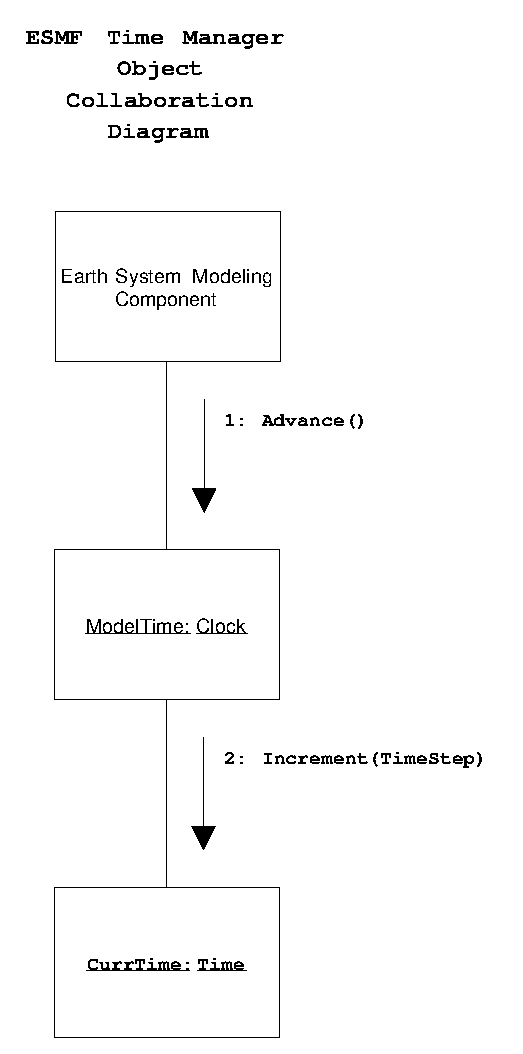
\includegraphics{TimeMgrOCD1.EPS}
   
Figure 3.  ESMF Time Manager Increment Model Time Scenario
   
\end{center}
